\section{QPSK Transmitter}

\begin{refsection}

\begin{tcolorbox}	
\begin{tabular}{p{2.75cm} p{0.2cm} p{10.5cm}} 	
\textbf{Student Name}  &:&  Andr\'e Mourato (2018/07/08 - 2018/07/08)\\
\textbf{Goal}          &:& ...\\
\textbf{Directory}     &:& sdf/qpsk\_transmitter
\end{tabular}
\end{tcolorbox}

This system simulates a QPSK transmitter~\cite{loudon2000}. A schematic representation of this system is shown in figure \ref{QPSK_transmitter_block_diagram_simple}.

\begin{figure}[h]
	\centering
	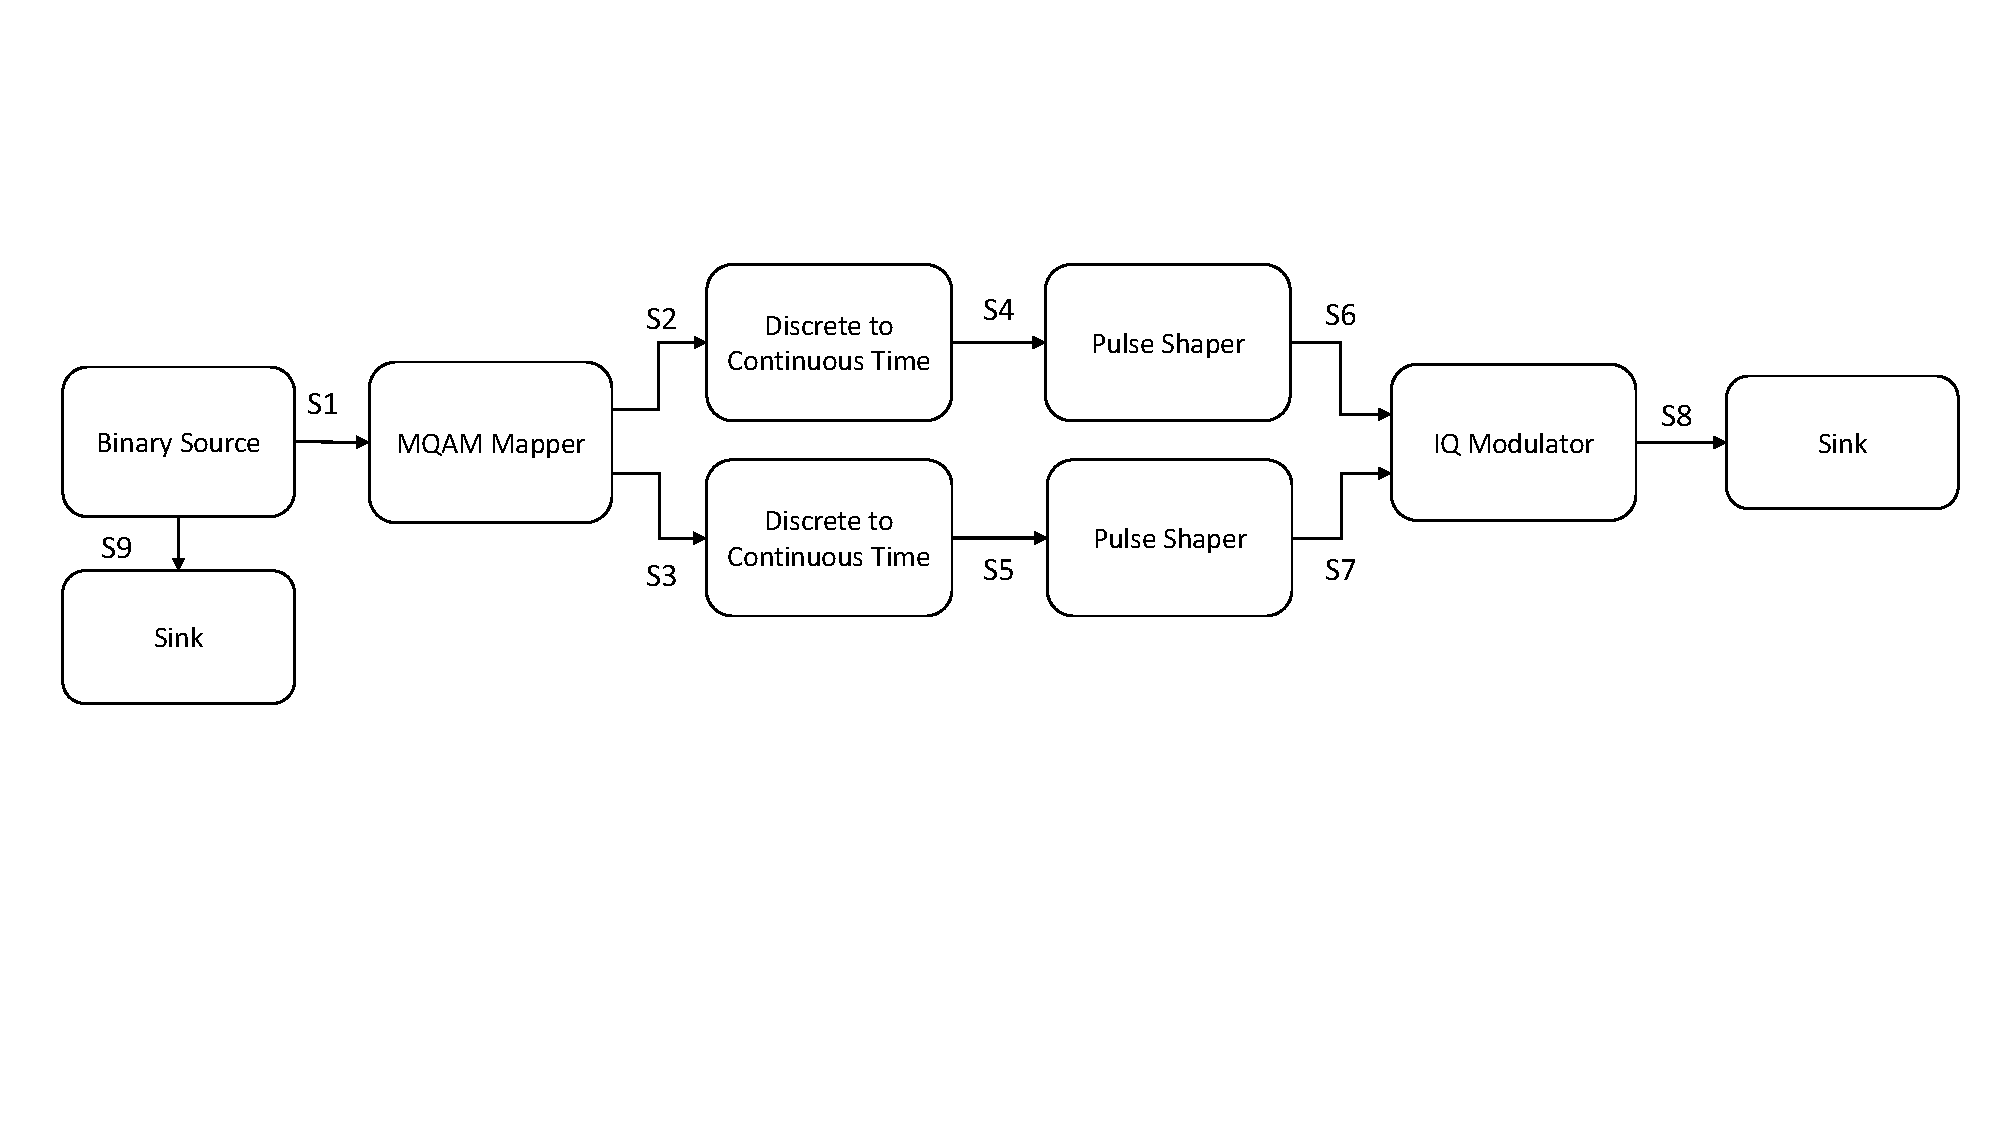
\includegraphics[width=1.0\textwidth]{./sdf/qpsk_transmitter/figures/qpsk_transmitter.pdf}
	\caption{QPSK transmitter block diagram.}\label{QPSK_transmitter_block_diagram_simple}
\end{figure}

\subsection*{Required files}\label{Required files}

\begin{table}[H]
\centering
\begin{tabulary}{1.0\textwidth}{|p{7.5cm}|p{6.5cm}|p{1cm}|}
\hline
\multicolumn{3}{|c|}{ \textbf{Header Files} } \\
\hline
\textbf{File}                    & \textbf{Comments} & \textbf{Status} \\ \hline
binary\_source\_20180523.h                 &                   & \checkmark \\ \hline
discrete\_to\_continuous\_time\_20180118.h &                   & \checkmark \\ \hline
iq\_modulator\_20180130.h                  &                   & \checkmark \\ \hline
m\_qam\_mapper\_20180118.h                 &                   & \checkmark \\ \hline
netxpto\_20180418.h                        &                   & \checkmark \\ \hline
pulse\_shaper\_20180118.h                  &                   & \checkmark \\ \hline
sink\_20180620.h                           &                   & \checkmark \\ \hline
\end{tabulary}
\end{table}		

\begin{table}[H]
\centering
\begin{tabulary}{1.0\textwidth}{|p{7.5cm}|p{6.5cm}|p{1cm}|}
\hline
\multicolumn{3}{|c|}{ \textbf{Source Files} } \\
\hline
\textbf{File}                      & \textbf{Comments} & \textbf{Status} \\ \hline
binary\_source\_20180523.cpp                 &                   & \checkmark \\ \hline
discrete\_to\_continuous\_time\_20180118.cpp &                   & \checkmark \\ \hline
iq\_modulator\_20180130.cpp                  &                   & \checkmark \\ \hline
m\_qam\_mapper\_20180118.cpp                 &                   & \checkmark \\ \hline
netxpto\_20180418.cpp                        &                   & \checkmark \\ \hline
pulse\_shaper\_20180118.cpp                  &                   & \checkmark \\ \hline
sink\_20180620.cpp                           &                   & \checkmark \\ \hline
\end{tabulary}
\end{table}	

\subsection*{System Input Parameters}

This system takes into account the following input parameters:

\begin{table}[H]
\centering
\begin{tabulary}{1.0\textwidth}{|p{4cm}|p{7cm}|p{4cm}|}
\hline
\multicolumn{3}{|c|}{ \textbf{System Input Parameters} } \\
\hline
\textbf{Parameter}     & \textbf{Default Value}                                     & \textbf{Comments} \\ \hline
sourceMode             & Random	                                                    & \\ \hline
patternLength          & 5                                                          & \\ \hline
bitStream              & ``0''                                                      & \\ \hline
bitPeriod              & $\frac{1}{50e9}$                                           & \\ \hline
iqAmplitude            & $\lbrace\lbrace\lbrace1,1\rbrace,\lbrace-1,1\rbrace,\lbrace-1,-1\rbrace,\lbrace1,-1\rbrace\rbrace\rbrace$ & \\ \hline
numberOfBits           & 1000                                                       & \\ \hline
numberOfSamplesPerSymbol & 16                                                       & \\ \hline
rollOffFactor          & 0.3                                                        & \\ \hline
impulseResponseTimeLength & 16                                                      & \\ \hline
bLength                & 16                                                         & \\ \hline
\end{tabulary}
\end{table}	


% bibliographic references for the section ----------------------------
\clearpage
\printbibliography[heading=subbibliography]
\end{refsection}
\addcontentsline{toc}{subsection}{Bibliography}
\cleardoublepage
% --------------------------------------------------------------------- 